\chapter{CapeVM}

This chapter we introduce the global design of CapeVM, which is based on Darjeeling \cite{Brouwers:2009cj}. It runs directly on the hardware, without any OS layer in between, and has complete control over the device. Like other sensor node VMs, Darjeeling is originally an interpreter. This interpreter was replaced with an AOT compiler: instead of interpreting the bytecode, CapeVM translates it to native code at load time, before the application is started. While JIT compilation is possible on some devices \cite{Ellul:2012thesis}, it depends on the ability to execute code from RAM, which many embedded CPUs, including the ATmega, cannot do.

\section{Goals}
\label{sec-CapeVM-goals}
Working on resource-constrained devices means we have to make some compromises. Our main goal is to build an AOT compiling VM that will produce safe code, performs well, and reduces the code size overhead seen in previous work. In addition, we want our VM to fit as many scenarios as possible, for example scenarios were multiple applications may be running on a single device. When new code is being loaded, the impact on other applications should be as small as possible.

WuKong, discussed in Section \ref{sec-state-of-the-art-wukong} is a good motivating example. Parts of WuKong applications may be written in Java. A node may be part of more than one application, and the WuKong master may dynamically decide to move an WuObject from one node to another. This means new Java code may have to be loaded onto a device, while parts of the same or another application are already running.

To support scenarios like this, the translation process should be very light weight. Specifically, it should use as little memory as possible, since this is a scarce resource and any memory used by the AOT compiler cannot be used for other concurrently running tasks. This means we cannot do any analysis on the bytecode that would require us to hold large data structures in memory.

Our goal is to limit memory use to around 100 bytes, which rules out most traditional AOT and JIT compiler techniques. It may be possible to do more complex optimisations to achieve even better performance through more complex optimisations, but, as we will see, much can be achieved even with very limited resources.

The two metrics we compromise on are load time and code size. Compiling to native code takes longer than simply storing bytecode and starting the interpreter, but we feel this load-time delay will be acceptable in many cases, and will be quickly compensated for by improved run-time performance. Native code is already larger than JVM bytecode, and our AOT compiled code is on average 78\% larger than its optimised C equivalent. This is the price we pay for increased performance, but the optimisations we propose do significantly reduce this code size overhead compared to previous work, thus reducing an important drawback of previous AOT compilation techniques.

We summarise our goals and constraints below:
\begin{itemize}
  \item Improve performance to within half of native optimised code.
  \item Provide the option to run applications in a safe, sandboxed environment.
  \item Keep memory consumption to around 100 bytes to allow concurrent tasks to keep running and maintain their state as new code is loaded onto the device.
  \item Limit code size overhead so the approach is feasible on mid-range sensor node devices: at least 64 KB of programme memory for 8-bit Atmel CPUs.
\end{itemize}

\section{Compilation process}
\label{sec-compilation-process}

\begin{figure}
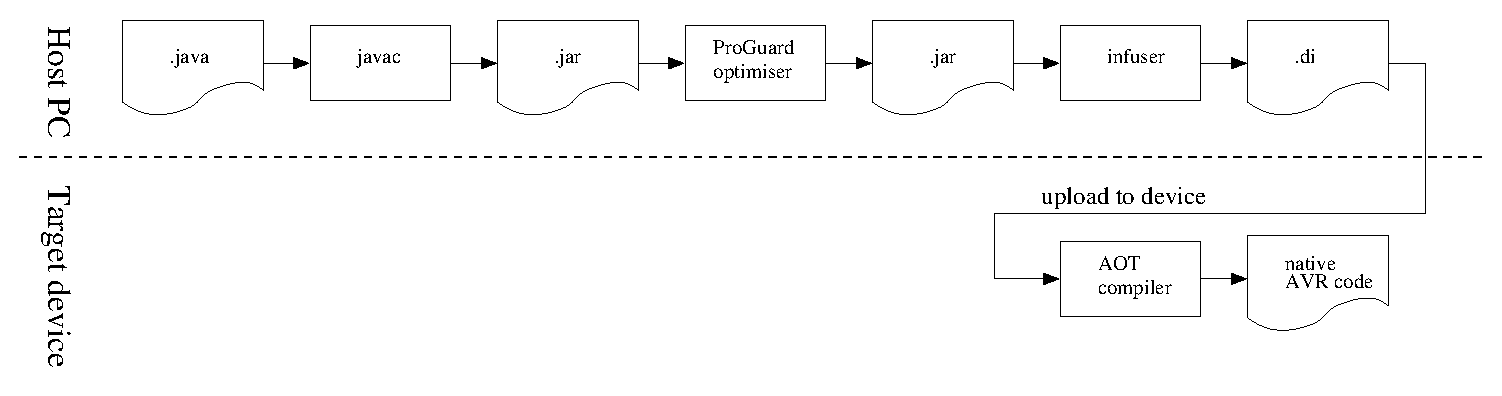
\includegraphics[width=\linewidth]{compilation-process.eps}
\caption{Java to native AVR compilation}
\label{fig-translation-process}
\end{figure}

The complete process from Java source to a native application on the node is shown in Figure \ref{fig-translation-process}. Like all sensor node JVMs, Darjeeling uses a modified JVM bytecode. Java source code is first compiled to normal Java classes. We then use ProGuard \cite{proguard} to optimise the bytecode, but these optimisations, while useful, are limited to very basic steps such as dead code removal, overlapping local variable slots where possible, etc.

The optimised Java classes are then transformed into Darjeeling's own bytecode format, called an \emph{infusion}. For details of this transformation we refer to the Darjeeling paper \cite{Brouwers:2009cj}. Here it is sufficient to note that no knowledge of the target platform is used in this transformation, so the result is still platform independent. This infusion is then sent to the node, where the AOT compiler translates it to native AVR code at load time.

When the node receives a large programme, it should not have to keep multiple messages in memory since this will consume too much memory. Our approach allows the bytecode to be translated to native code in a single pass, on instruction at a time. Only some small, fixed-size data structures are kept in memory during the process. A second pass over the generated code then fills in addresses left blank by branch instructions, since the target addresses of forward branches are not known until the target instruction is generated.

This means each message, which can be as small as a single bytecode instruction, can be freed immediately after processing. Since messages do need to be processed in the correct order, the actual transmission protocol may still decide to keep more messages in memory to reduce the need for retransmissions in the case of out of order delivery. But the translation process does not require it to do so, and a protocol that values memory usage over retransmissions cost could simply discard out of order messages and request retransmissions when necessary.


\section{Translating bytecode to native code}
\label{sec-basic-translation}

\begin{table}
\caption{Translation of \mycode{ do{A>>>=1;} while(A>B);}}
\label{tbl-basic-translation}
    \scriptsize
    \begin{tabular}{llll} % NO SIMULATION DATA
    \toprule
    Bytecode            & AOT compiler                       & native code & cycles \\
    \midrule
    \midrule
    0: BRTARGET(0)      & \sccomment{record current address} &            & \\
    1: SLOAD\_0         & emit\_LDD(R1,Y+0)                  & LDD R1,Y+0 & 4 \\
                        & emit\_PUSH(R1)                     & PUSH R1    & 4 \\
    2: SCONST\_1        & emit\_LDI(R1,1)                    & LDI R1,1   & 2 \\
                        & emit\_PUSH(R1)                     & MOV R2,R1  & 1 \\
    3: SUSHR            & emit\_POP(R2)                      &            & \\
                        & emit\_POP(R1)                      & POP R1     & 4 \\
                        & emit\_RJMP(+2)                     & RJMP +2    & 2 \\
                        & emit\_LSR(R1)                      & LSR R1     & 2 \\
                        & emit\_DEC(R2)                      & DEC R2     & 2 \\
                        & emit\_BRPL(-2)                     & BRPL -2    & 3 \\
                        & emit\_PUSH(R1)                     &            & \\
    4: SSTORE\_0        & emit\_POP(R1)                      &            & \\
                        & emit\_STD(Y+0,R1)                  & STD Y+0,R1 & 4 \\
    5: SLOAD\_0         & emit\_LDD(R1,Y+0)                  & LDD R1,Y+0 & 4 \\
                        & emit\_PUSH(R1)                     & PUSH R1    & 4 \\
    6: SLOAD\_1         & emit\_LDD(R1,Y+2)                  & LDD R1,Y+2 & 4 \\
                        & emit\_PUSH(R1)                     &            & \\
    7: IF\_SCMPGT(BT:0) & emit\_POP(R1)                      &            & \\
                        & emit\_POP(R2)                      & POP R2     & 4 \\
                        & emit\_CP(R1,R2)                    & CP R1,R2   & 2 \\
                        & emit\_branchtag(GT,0)              & BRGT 0:    & 2 (taken), \\
                        &                                    &            & or 1 (not taken) \\
    \bottomrule
    \end{tabular}
\end{table}

The baseline AOT compiler is an implementation of Ellul's approach, as described in his thesis \cite{Ellul:2012thesis}, adapted for the Atmel ATmega128 CPU, while Ellul's work uses the Texas Instruments MSP430. 

In this unoptimised version of the translator, each bytecode instruction the VM receives is simply replaced with a fixed, equivalent sequence of native instructions. The native stack is used to mimic the VM's operand stack. An example of this is shown in Table \ref{tbl-basic-translation}.

The first column shows a fragment of bytecode which does a shift right of 16-bit variable \mycode{A}, and repeats this while \mycode{A} is greater than \mycode{B}. While this may not be a very useful operation, it is the smallest example that will allow us to illustrate our code generation optimisations in the following chapter. The second column shows the code the AOT compiler will execute for each bytecode instruction. Together, the first and second column match the case labels and body of a big switch statement in the compiler. The third column shows the resulting AVR native code, which is currently almost a 1-on-1 mapping, with the exception of the branch instruction and some optimisations by a simple peephole optimiser, both described below.

The example has been slightly simplified for readability. Since the AVR is an 8-bit CPU, in the real code many instructions are duplicated for the high and low bytes. The cycle count is based on the actual number of generated instructions, and for a single iteration.

\subsection{Branches}
Forward branches pose a problem for this direct translation approach since the target address is not yet known. A second problem is that on the ATmega, a branch may take 1 to 3 words, depending on the distance to the target, so it is also not known how much space should be reserved for a branch.

To solve this the infuser modifies the bytecode by inserting a new instruction, \mycode{BRTARGET}, in front of any instruction that is the target of a branch. The branch instructions themselves are modified to target the id of a \mycode{BRTARGET}, which are implicitly numbered, instead of a bytecode offset. When the VM encounters a \mycode{BRTARGET} during translation, no code is emitted, but the address where the next instruction will be emitted is recorded in a separate part of flash memory. Branch instruction initially emit a temporary 3-word 'branch tag', containing the branch target id and the branch condition. After code generation is finished and all target addresses are known, the VM scans the generated code a second time, and replaces each branch tag with the real branch instruction.

There is still the matter of the different sizes a branch may take. The VM could simply add \mycode{NOP} instructions to smaller branches to keep the size of each branch at 3 words, but this causes both a code size penalty and a performance penalty on small, non-taken branches. Instead, the VM does another scan of the code, before replacing the branch tags, to update the branch target addresses by compensating for cases where a smaller branch will be used. This second scan adds about 500 bytes to the VM, but improves performance, especially on benchmarks where branches are common.

This is an example of something we often see: an optimisation may take a few hundred bytes to implement, but its usefulness may depend on the characteristics of the code being run. In this work we usually decided to implement these optimisations, since in many cases, including this one, they also result in smaller generated code.

\subsection{Darjeeling split-stack architecture}
\label{sec-darjeeling-split-architecure}

\begin{figure}
\centering
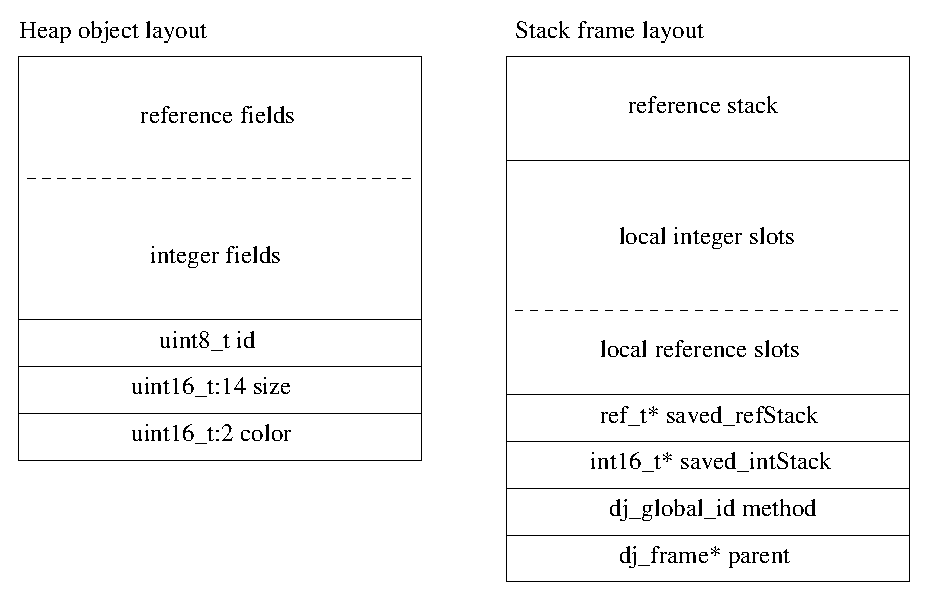
\includegraphics[width=0.8\linewidth]{object-and-stack-frame-layout.eps}
\caption{Infusion, object and stack frame layout}
\label{fig-object-and-stack-frame-layout}
\end{figure}

When Darjeeling's garbage collector runs, it needs to mark the \emph{root set}: the set of all live, directly reachable objects. This is then iteratively expanded to also cover all indirectly reachable objects. For example in Figure \ref{fig-jvm-memory}, only the two objects on the left of the heap are in the root set, two others are also reachable but not in the root set, while the fifth is not reachable and will be freed by the garbage collector.

To mark the root set, the garbage collector needs to determine which local variables, static variables, object fields, and values on the operand stack are references. To do this efficiently, Darjeeling separates references and integers throughout the VM: the operand stack, instance variables on the heap, class static variables, and local variables in a method's stack frame are all split in a block for integers and one for references, as shown in Figure \ref{fig-object-and-stack-frame-layout}.

In our AOT compiler we use the native stack for the VM's integer operand stack, so the integer operand stack is not in a method's stack frame, but the reference stack is. This uses less memory than having the integer stack in the stack frame, since we need to reserve space for the maximum stack depth in the frame, which is often much lower for the reference stack than for the integer stack. We use the AVR's X register as an extra stack pointer for the reference stack.

\subsection{Peephole optimisation}
\begin{table}
\caption{CapeVM's peephole optimisations}
\label{tbl-CapeVM-peephole}
    \begin{threeparttable}
    \begin{tabular}{lrrlrr} % NO SIMULATION DATA
    \toprule
    Before         & Cycles & Bytes   & After        & Cycles & Bytes   \\
    Instructions   &        &         & Instructions &        &         \\
    \midrule
    \midrule
    PUSH Rx        & 4      & 4       &              & 0      & 0 \\
    POP Rx         &        &         &              &        & \\
    \midrule
    PUSH Rx        & 4      & 4       & MOV Ry, Rx   & 1      & 2 \\
    POP Ry         &        &         &              &        & \\
    \midrule
    ST X+, Rx      & 4      & 4       &              & 0      & 0 \\
    LD -X, Rx      &        &         &              &        & \\
    \midrule
    ST X+, Rx      & 4      & 4       & MOV Ry, Rx   & 1      & 2 \\
    LD -X, Ry      &        &         &              &        & \\
    \midrule
    MOV Ry, Rx     & 2      & 4       & MOVW Ry, Rx  & 1      & 2 \\
    MOV Ry+1, Rx+1 &        &         &              &        & \\
    \bottomrule
    \end{tabular}
    \begin{tablenotes}
    \item The X register is used as the reference stack pointer.
    \end{tablenotes}
    \end{threeparttable}
\end{table}

Since the baseline should be as close as possible to Ellul's MSP430 implementation, a similar set of peephole optimisations were implemented. However, differences between the ATmega and MSP430 instruction sets means they are not completely identical. The complete set of peephole optimisations in CapeVM is shown in Table \ref{tbl-CapeVM-peephole}.

A \mycode{push} directly followed by a \mycode{pop} are both either eliminated or replaced by a \mycode{mov}. A push or pop may be either a real \mycode{push} or \mycode{pop} instruction for the integer stack, or implemented using a \mycode[c-objdump]{st X+} or \mycode[c-objdump]{ld -X} instruction for the reference stack. Both cases are optimised in the same way. We also similarly optimise blocks of pushes followed by blocks of pops, which are very common on the 8-bit ATmega. 

When the push and pop instructions target different registers, this results in multiple \mycode{mov} instructions. Two \mycode{mov} instructions with consecutive registers can be further optimised using the \mycode{movw} instruction to copy a register pair to another register pair in a single cycle.


\subsection{Bytecode modification}
\label{sec-vm-design-bytecode-modifications}
We made several modifications to the infuser and introduced new bytecode instructions to support our AOT compiler and improve performance. These changes will be introduced in more detail in the following sections, but for completeness we also list them here:

\begin{itemize}
	\item The \mycode{BRTARGET} opcode marks targets of branch instructions. All branch instructions are modified to target a \mycode{BRTARGET} id instead of a bytecode offset.
	\item The \mycode{MARKLOOP} opcode marks inner loops and the variables they use.
	\item \mycode{PUTFIELD_A_FIXED} and \mycode{GETFIELD_A_FIXED} are used to access an object's reference fields when the offset is known at compile time. The offset ia always known at compile time for integer fields.
	\item The \mycode{SIMUL} opcode does 16x16-bit to 32-bit multiplication.
	\item New \mycode{_CONST} versions of the (variable) bit shift opcodes support shifting by a constant number of bits.
	\item The \mycode{INVOKELIGHT} opcode supports an optimised 'lightweight' way of calling methods.
	\item The \mycode{GETCONSTARRAY} opcodes support reading from arrays of constant data stored in the constant pool.
	\item Array access opcodes use 16-bit instead of 32-bit indexes.
\end{itemize}


\section{Limitations}
Since our compiler is based on Darjeeling, we share its limitations, most notably a lack of floating point support and reflection. In addition, we do not support threads or exceptions because after compilation to native code, we lose the interpreter loop as a convenient place to switch between threads or unwind the stack to jump to an exception handler. Threads and exceptions have been implemented in Ellul's AOT compiler \cite{Ellul:2012thesis}, proving it is possible to add support for both, but we feel the added complexity in an environment where code space is at a premium makes other, more lightweight models for concurrency and error handling more appropriate.

We will discuss the cost of using our VM more in more detail in Chapter \ref{sec-evaluation}, and alternatives to some traditional JVM features in Chapter \ref{sec-lessons-from-jvm}.


\section{Target platforms}
CapeVM was implemented for the ATmega128 CPU \cite{Atmel:ATmega128Datasheet}. The AVR family of CPUs is widely used in low power embedded systems and sensor nodes. However, our approach does not depend on any AVR specific properties and we expect similar results for many other CPUs in this class. The main requirements are the ability to reprogramme its own programme memory, and the availability of a sufficient number of registers.

The ATmega128 has 32 8-bit registers. We expect the Cortex M0 \cite{ARM:2009vz}, with 13 32-bit general purpose registers, or the MSP430 \cite{TexasInstrumentsIncorporated:MSP430F1611Datasheet}, with 12 16-bit registers, and used by Ellul and Martinez \cite{Ellul:2010iw}, to both be good matches as well. In Section \ref{sec-evaluation-other-platforms} we will examine the expected impact of the number of registers and of using a 16-bit or 32-bit architecture on the resulting performance.
